\chapter{Chemical Bonding}

\section{Introduction}
A \textit{chemical bond} is a mutual attraction between the nuclei and valence
electrons of different atoms that binds the atoms together.  Atoms form chemical
bonds to gain a greater stability.

In the formation of a bond, atoms share, or give up, their valenece electrons.
This sharing results in a greater stability as a whole for the system.  The way
in which the electrons are shared is determinant of the type of bond that is
formed.

\section{Ionic Bonds}
Ionic bonding occurs from the electrical attraction between large numbers of
positive, and negatively charged ions.  The difference in electronegativity
determines what type of bond it is.

\begin{description}
  \item[Ionic] difference in electronegativity between 1.7 and 3.3.
  \item[Molecular (Polar)] difference in electronegativity between 0.3 and 1.7.
  \item[Molecular (Nonpolar)] difference in electronegativity between 0 and 0.3.
\end{description}

\section{Covalent Bonds}
Covalent bonds represents the sharing of electron pairs between two atoms.

\subsection{Non-polar covalent bonds}
These bonds are covalent bonds in which the bonding electrons are shared equally
between the bonded atoms, creating a balanced distribution of charge.  They
are 0 to 5\% ionic character and have an electronegativity difference of 0 to
0.3.

\subsection{Polar covalent bonds}
Bonds that are 5 to 50\% percent ionic in character have an uneven distribution
of charge, such that the bonded atoms have an unequal attraction for the shared
electrons.

\section{Terminology}
\begin{description}
  \item[Molecule] a neutral group of atoms that are held together by covalent
    bonds
  \item[Molecular compound] a chemical compound where the simplest unit is
    molecules
  \item[Chemical Formula] indicates the relative number of atoms of each kind in
    a chemical compound using atomic symbols and numerical subscripts
\end{description}

\section{Motivation}
Why form a bond?  To answer this question, we must first understand the
motivation of atoms.  All atoms seek to become the most chemically stable that
they can be, and if they can lose, gain, or share a valence electron in order to
do so, they will.

However, bonded atoms behave not as one might initially assume.  Two atoms which
are far away initially have no force of attraction, however, as they get closer,
this force increases and increases, until they are \textit{too} close and thus
begin to repel each other.  As the atoms back off each other, they are again
attracted, and thus vibrate in this state of flux.

\begin{figure}[H]
  \centering
  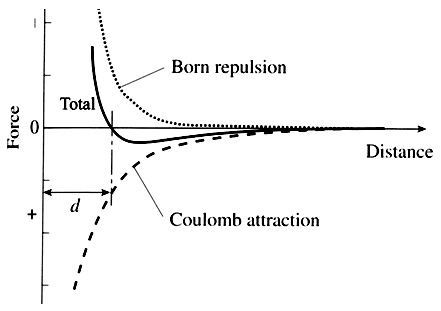
\includegraphics{res/ionic_bond_length.jpg}
  \caption{The repulsion of two ionically bonded atoms at different lengths}
\end{figure}

When forming a bond, some energy is released.  This same amount of energy must
again be added to the bonded compound to break those bonds.  Some notes on the above diagram follow:

\begin{description}
  \item[Bond length] the distance between two bonded atoms at their minimum
    potential energy.  Or, the average distance between two bonded atoms.  This
    is the local min of the above graph.
  \item[Bond energy] the amount of energy required to break a chemical bond to
    form neutral isolated atoms.  This is the local max at the right-hand side
    of the graph.
\end{description}

\subsection{Bonding of Electrons}
The \textit{octet rule} states that chemical compounds will tend to form such
that each atom, by either gaining, losing, or sharing electrons has an octet of
electrons in its highest occupied energy level.

\subsubsection{Exceptions}
\begin{itemize}
  \item Hydrogen does not form an octet, it only has two electrons around it.
  \item Boron \& aluminum do not form octets, they have a total of 6 electrons
    surrounding them.
  \item Some p-block elements have more than 8 electrons.
\end{itemize}

\section{Representation}
\subsection{Electron-Dot Structure}
The \textit{electron-dot structure} shows the amount of valence electrons around
an atom.  You only draw the dots of the valence electrons, and they are drawn
around the chemical symbol of that element.

\begin{figure}[H]
  \centering
  
\includegraphics{res/electron_dot_structure.jpg}
\end{figure}

\subsection{Lewis Dot Structure}
The Lewis Dot Structure hinges on this idea of electron-dot structures, but
extends it to molecules.  Lewis Structures are formulae in which atomic symbols
represent nuclei and inner-shell electrons.  Dot-pairs or dashes between two
atomic symbols represents the electron pair in bonds, and dots adjacent to only
one atomic symbol represent unshared electrons.

\begin{description}
  \item[Lone pair] a pair of electrons that is not involved in bonding and
    belongs to only one atom
  \item[Structural formulae] indicates the kind, number, arrangement, and bonds
    but not the lone pairs of atoms in a molecule.
\end{description}

To generate a Lewis Dot Structure, take the following steps:

\begin{enumerate}
  \item Determine the type and number of atoms in the molecule
  \item Write the electron-dot structure for each atom in the molecule
  \item Determine the total number of valence electrons in the atom to be
    combined
  \item Arrange the atoms to form a skeletal structure for the molecule.
    \textit{Carbon is always the central atom in these structure if present, but
    otherwise pick the least-electronegative atom, and not hydrogen}
  \item Connect the atoms by electron-pair bonds
  \item Add unshared pairs of electrons so that each hydrogen atom shares a pair
    of electrons and each non-metal has a full octet
\end{enumerate}

\begin{figure}[H]
  \centering
  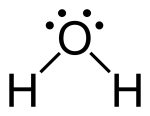
\includegraphics{res/lewis_structure_water.png}
  \caption{A Lewis dot-structure representation of a \textit{Chlorine} ion}
\end{figure}

\section{Bonding and Bonds}
\begin{description}
  \item[Single bond] a covalent bond produced by the sharing of one pair of
    electrons between two atoms
  \item[Double bond] a covalent bond produced by the sharing of two pairs of
    electrons between two atoms
  \item[Triple bond] a covalent bond produced by the sharing of three pairs of
    electrons between two atoms
\end{description}

\subsection{Resonance Structures}
Sometimes, the Lewis Dot Structure does not accurately represent a molecule or
ion.  For example, in the case of \ce{O3} \textit{(ozone)}, several different
structures can occur.  This is called resonance, and cannot be captured by
traditional Lewis structures.

Since the double bond can occur in multiple places (but only one place at a
time) the Lewis structure is not suited to correctly display this.  In the
example below, the double-bond in the polyatomic ion \textit{nitrate} is shown
in multiple places throughout the structure.

\begin{figure}[H]
  \centering
  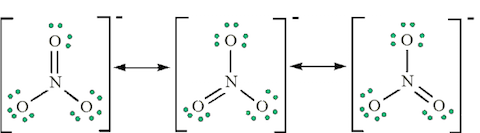
\includegraphics{res/nitrate_resonance.png}
  \caption{The double bond in this ion is placed in multiple locations
  throughout the diagram, to show that it can exist in more than one spot.}
\end{figure}

\subsection{Metallic Bonds}
A \textit{metallic bond} is the result of the attraction between metal atoms and
the surroudning sea of electrons.  It is acountable for most of the unique
behavior of metals.

\section{Molecular Geometry}
While Lewis structures are all well and good, their major drawback is that they
are only 2-dimensional.  Molecular geometry is important because we can
determine the molecular polarity or uneven distibution of molecular charge
through structures in 3-dimensions.

\subsection{VSEPR Theory}
VSPER Theory states that the repulsion between sets of valence-level electrons
surrounding an atom causes these sets to be oriented as far apart as possible.

\begin{figure}[H]
  \centering
  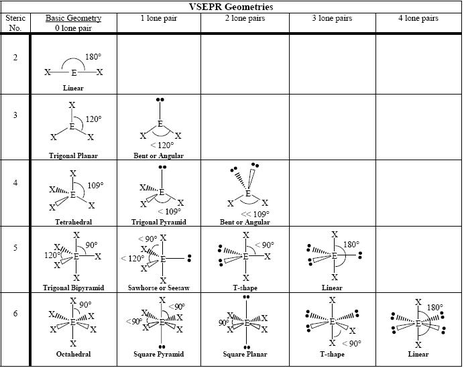
\includegraphics{res/vsepr_chart.png}
\end{figure}
